\documentclass{standalone}
\usepackage{xcolor}
\usepackage{tikz}
\usetikzlibrary{positioning, shapes.multipart, calc, graphs, graphs.standard}
\begin{document}
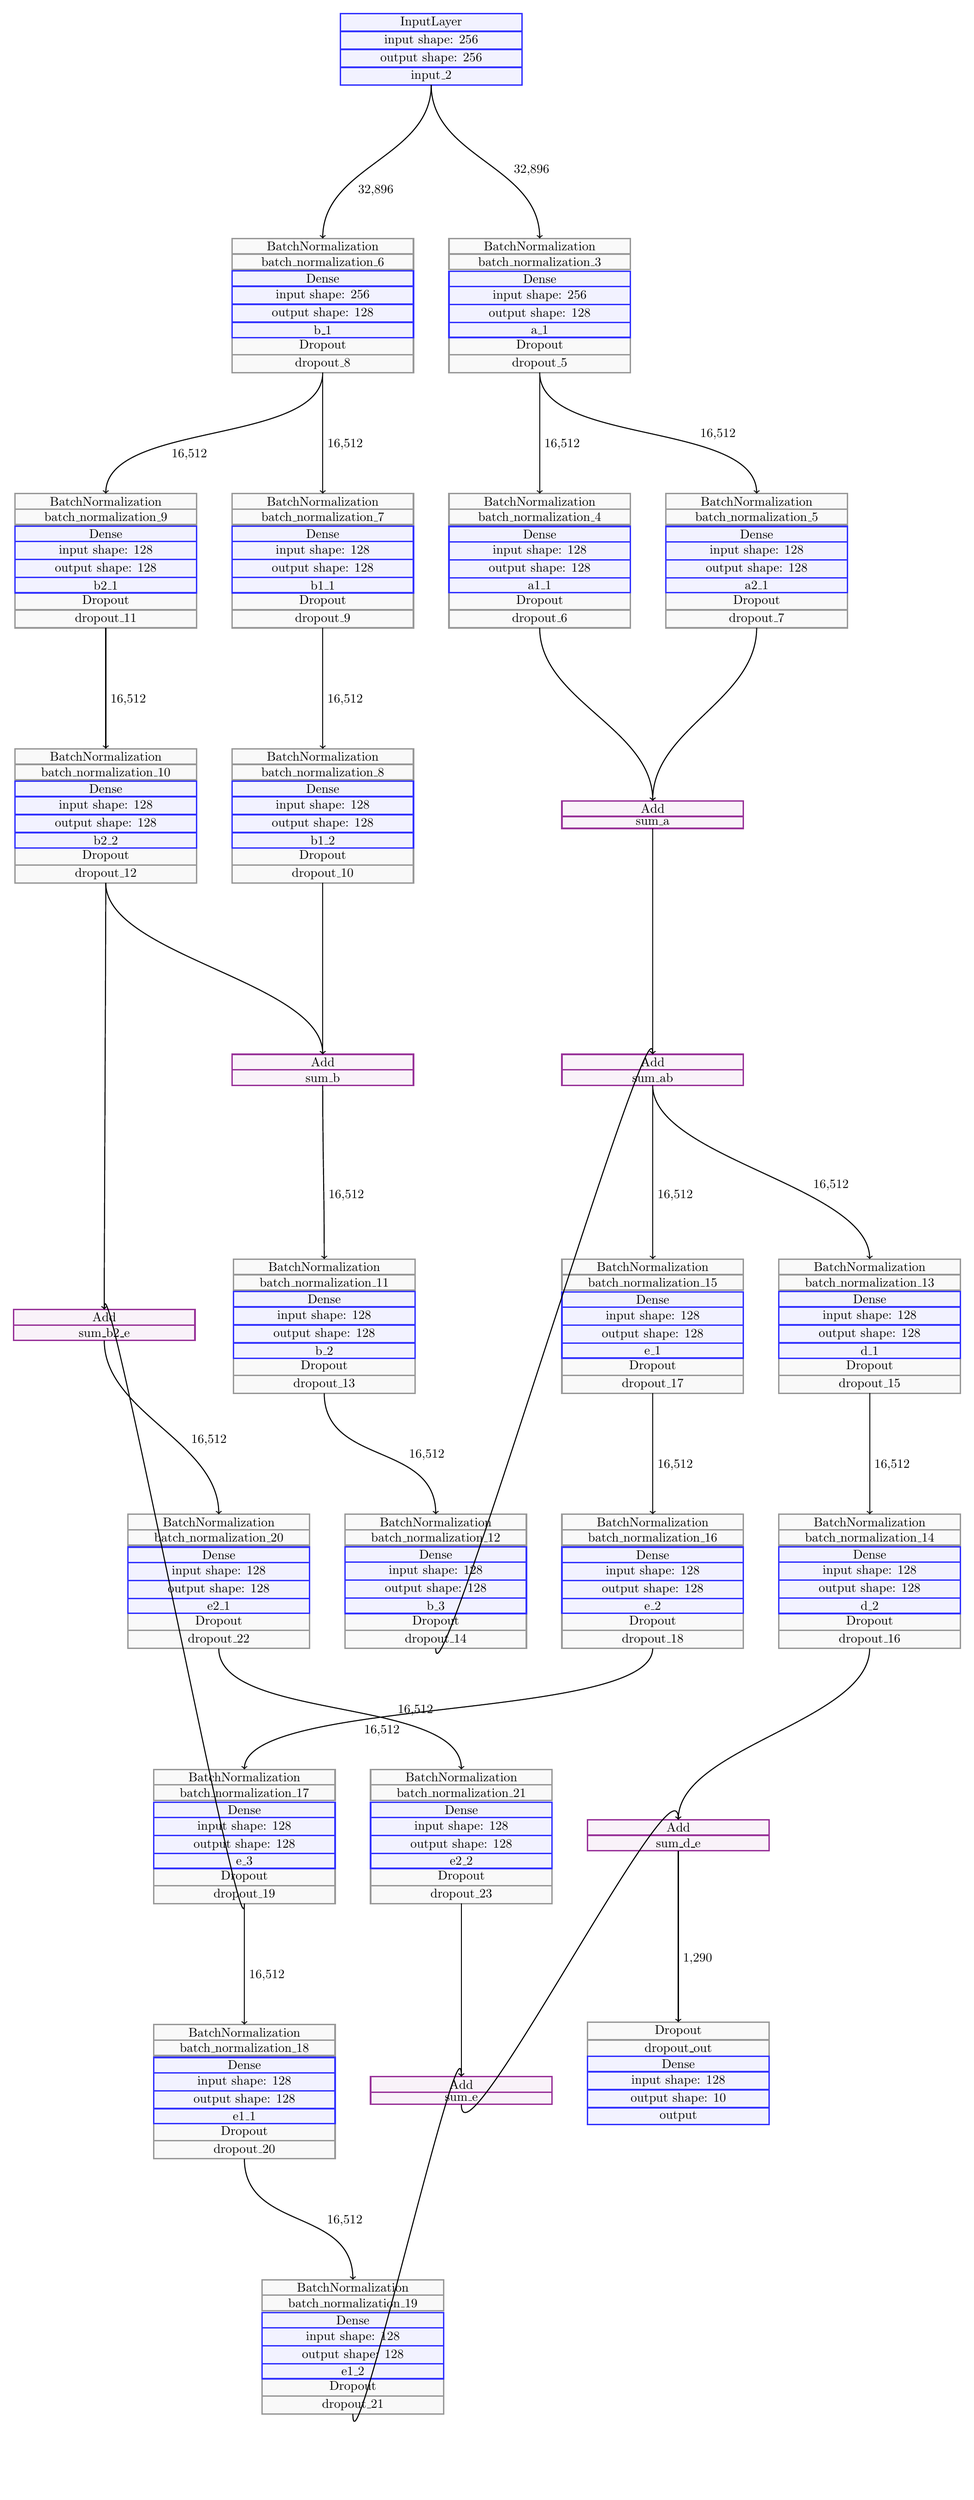
\begin{tikzpicture}[x=30pt, y=30pt]
% style: major_grid
\tikzstyle{major_grid}=[black,step=20pt]
% style: minor_grid
\tikzstyle{minor_grid}=[very thin,step=10pt]
% style: defaultEdge
\tikzstyle{defaultEdge}=[thick,out=-90,in=90,out distance=2cm,in distance=2cm]
% style: defaultLabel
\tikzstyle{defaultLabel}=[auto,pos=0.65]
% style: OperationLayer_style
\tikzstyle{OperationLayer_style}=[rectangle split,rectangle split ignore empty parts,very thick,rectangle split parts=5,draw=violet!80,fill=violet!5,minimum width=5cm,outer sep=0cm,inner sep=2pt]
% style: UtilityLayer_style
\tikzstyle{UtilityLayer_style}=[rectangle split,rectangle split ignore empty parts,very thick,rectangle split parts=5,draw=gray!80,fill=gray!5,minimum width=5cm,outer sep=0cm,inner sep=2pt]
% style: TrainableLayer_style
\tikzstyle{TrainableLayer_style}=[rectangle split,rectangle split ignore empty parts,very thick,rectangle split parts=5,draw=blue!80,fill=blue!5,minimum width=5cm,outer sep=0cm,inner sep=2pt]

% node group: input_2_group
% node: input_2
\node[TrainableLayer_style] (input_2) at (8.543307086614174, 60.0)
    {
    \nodepart{one}{InputLayer}
    \nodepart{two}{input shape: 256}
    \nodepart{three}{output shape: 256}
    \nodepart{four}{input\_2}};
% end of node group: input_2_group

% node group: b_1_group
% node: batch_normalization_6
\node[UtilityLayer_style] (batch_normalization_6) at (5.708661417322834, 54.64999999999999)
    {
    \nodepart{one}{BatchNormalization}
    \nodepart{two}{batch\_normalization\_6}};
% node: dropout_8
\node[UtilityLayer_style] (dropout_8) at (5.708661417322834, 52.016666666666666)
    {
    \nodepart{one}{Dropout}
    \nodepart{two}{dropout\_8}};
% node: b_1
\node[TrainableLayer_style] (b_1) at (5.708661417322834, 53.33333333333333)
    {
    \nodepart{one}{Dense}
    \nodepart{two}{input shape: 256}
    \nodepart{three}{output shape: 128}
    \nodepart{four}{b\_1}};
% end of node group: b_1_group

% node group: a_1_group
% node: batch_normalization_3
\node[UtilityLayer_style] (batch_normalization_3) at (11.377952755905511, 54.64999999999999)
    {
    \nodepart{one}{BatchNormalization}
    \nodepart{two}{batch\_normalization\_3}};
% node: dropout_5
\node[UtilityLayer_style] (dropout_5) at (11.377952755905511, 52.016666666666666)
    {
    \nodepart{one}{Dropout}
    \nodepart{two}{dropout\_5}};
% node: a_1
\node[TrainableLayer_style] (a_1) at (11.377952755905511, 53.33333333333333)
    {
    \nodepart{one}{Dense}
    \nodepart{two}{input shape: 256}
    \nodepart{three}{output shape: 128}
    \nodepart{four}{a\_1}};
% end of node group: a_1_group

% node group: b1_1_group
% node: batch_normalization_7
\node[UtilityLayer_style] (batch_normalization_7) at (5.708661417322834, 47.98333333333333)
    {
    \nodepart{one}{BatchNormalization}
    \nodepart{two}{batch\_normalization\_7}};
% node: dropout_9
\node[UtilityLayer_style] (dropout_9) at (5.708661417322834, 45.35)
    {
    \nodepart{one}{Dropout}
    \nodepart{two}{dropout\_9}};
% node: b1_1
\node[TrainableLayer_style] (b1_1) at (5.708661417322834, 46.666666666666664)
    {
    \nodepart{one}{Dense}
    \nodepart{two}{input shape: 128}
    \nodepart{three}{output shape: 128}
    \nodepart{four}{b1\_1}};
% end of node group: b1_1_group

% node group: b2_1_group
% node: batch_normalization_9
\node[UtilityLayer_style] (batch_normalization_9) at (0.03937007874015748, 47.98333333333333)
    {
    \nodepart{one}{BatchNormalization}
    \nodepart{two}{batch\_normalization\_9}};
% node: dropout_11
\node[UtilityLayer_style] (dropout_11) at (0.03937007874015748, 45.35)
    {
    \nodepart{one}{Dropout}
    \nodepart{two}{dropout\_11}};
% node: b2_1
\node[TrainableLayer_style] (b2_1) at (0.03937007874015748, 46.666666666666664)
    {
    \nodepart{one}{Dense}
    \nodepart{two}{input shape: 128}
    \nodepart{three}{output shape: 128}
    \nodepart{four}{b2\_1}};
% end of node group: b2_1_group

% node group: a1_1_group
% node: batch_normalization_4
\node[UtilityLayer_style] (batch_normalization_4) at (11.377952755905511, 47.98333333333333)
    {
    \nodepart{one}{BatchNormalization}
    \nodepart{two}{batch\_normalization\_4}};
% node: dropout_6
\node[UtilityLayer_style] (dropout_6) at (11.377952755905511, 45.35)
    {
    \nodepart{one}{Dropout}
    \nodepart{two}{dropout\_6}};
% node: a1_1
\node[TrainableLayer_style] (a1_1) at (11.377952755905511, 46.666666666666664)
    {
    \nodepart{one}{Dense}
    \nodepart{two}{input shape: 128}
    \nodepart{three}{output shape: 128}
    \nodepart{four}{a1\_1}};
% end of node group: a1_1_group

% node group: a2_1_group
% node: batch_normalization_5
\node[UtilityLayer_style] (batch_normalization_5) at (17.04724409448819, 47.98333333333333)
    {
    \nodepart{one}{BatchNormalization}
    \nodepart{two}{batch\_normalization\_5}};
% node: dropout_7
\node[UtilityLayer_style] (dropout_7) at (17.04724409448819, 45.35)
    {
    \nodepart{one}{Dropout}
    \nodepart{two}{dropout\_7}};
% node: a2_1
\node[TrainableLayer_style] (a2_1) at (17.04724409448819, 46.666666666666664)
    {
    \nodepart{one}{Dense}
    \nodepart{two}{input shape: 128}
    \nodepart{three}{output shape: 128}
    \nodepart{four}{a2\_1}};
% end of node group: a2_1_group

% node group: sum_a_group
% node: sum_a
\node[OperationLayer_style] (sum_a) at (14.330708661417322, 40.0)
    {
    \nodepart{one}{Add}
    \nodepart{two}{sum\_a}};
% end of node group: sum_a_group

% node group: b1_2_group
% node: batch_normalization_8
\node[UtilityLayer_style] (batch_normalization_8) at (5.708661417322834, 41.31666666666666)
    {
    \nodepart{one}{BatchNormalization}
    \nodepart{two}{batch\_normalization\_8}};
% node: dropout_10
\node[UtilityLayer_style] (dropout_10) at (5.708661417322834, 38.68333333333334)
    {
    \nodepart{one}{Dropout}
    \nodepart{two}{dropout\_10}};
% node: b1_2
\node[TrainableLayer_style] (b1_2) at (5.708661417322834, 40.0)
    {
    \nodepart{one}{Dense}
    \nodepart{two}{input shape: 128}
    \nodepart{three}{output shape: 128}
    \nodepart{four}{b1\_2}};
% end of node group: b1_2_group

% node group: b2_2_group
% node: batch_normalization_10
\node[UtilityLayer_style] (batch_normalization_10) at (0.03937007874015748, 41.31666666666666)
    {
    \nodepart{one}{BatchNormalization}
    \nodepart{two}{batch\_normalization\_10}};
% node: dropout_12
\node[UtilityLayer_style] (dropout_12) at (0.03937007874015748, 38.68333333333334)
    {
    \nodepart{one}{Dropout}
    \nodepart{two}{dropout\_12}};
% node: b2_2
\node[TrainableLayer_style] (b2_2) at (0.03937007874015748, 40.0)
    {
    \nodepart{one}{Dense}
    \nodepart{two}{input shape: 128}
    \nodepart{three}{output shape: 128}
    \nodepart{four}{b2\_2}};
% end of node group: b2_2_group

% node group: sum_ab_group
% node: sum_ab
\node[OperationLayer_style] (sum_ab) at (14.330708661417322, 33.333333333333336)
    {
    \nodepart{one}{Add}
    \nodepart{two}{sum\_ab}};
% end of node group: sum_ab_group

% node group: sum_b_group
% node: sum_b
\node[OperationLayer_style] (sum_b) at (5.708661417322834, 33.333333333333336)
    {
    \nodepart{one}{Add}
    \nodepart{two}{sum\_b}};
% end of node group: sum_b_group

% node group: sum_b2_e_group
% node: sum_b2_e
\node[OperationLayer_style] (sum_b2_e) at (0.0, 26.666666666666664)
    {
    \nodepart{one}{Add}
    \nodepart{two}{sum\_b2\_e}};
% end of node group: sum_b2_e_group

% node group: e_1_group
% node: batch_normalization_15
\node[UtilityLayer_style] (batch_normalization_15) at (14.330708661417322, 27.98333333333333)
    {
    \nodepart{one}{BatchNormalization}
    \nodepart{two}{batch\_normalization\_15}};
% node: dropout_17
\node[UtilityLayer_style] (dropout_17) at (14.330708661417322, 25.349999999999998)
    {
    \nodepart{one}{Dropout}
    \nodepart{two}{dropout\_17}};
% node: e_1
\node[TrainableLayer_style] (e_1) at (14.330708661417322, 26.666666666666664)
    {
    \nodepart{one}{Dense}
    \nodepart{two}{input shape: 128}
    \nodepart{three}{output shape: 128}
    \nodepart{four}{e\_1}};
% end of node group: e_1_group

% node group: d_1_group
% node: batch_normalization_13
\node[UtilityLayer_style] (batch_normalization_13) at (20.0, 27.98333333333333)
    {
    \nodepart{one}{BatchNormalization}
    \nodepart{two}{batch\_normalization\_13}};
% node: dropout_15
\node[UtilityLayer_style] (dropout_15) at (20.0, 25.349999999999998)
    {
    \nodepart{one}{Dropout}
    \nodepart{two}{dropout\_15}};
% node: d_1
\node[TrainableLayer_style] (d_1) at (20.0, 26.666666666666664)
    {
    \nodepart{one}{Dense}
    \nodepart{two}{input shape: 128}
    \nodepart{three}{output shape: 128}
    \nodepart{four}{d\_1}};
% end of node group: d_1_group

% node group: b_2_group
% node: batch_normalization_11
\node[UtilityLayer_style] (batch_normalization_11) at (5.748031496062992, 27.98333333333333)
    {
    \nodepart{one}{BatchNormalization}
    \nodepart{two}{batch\_normalization\_11}};
% node: dropout_13
\node[UtilityLayer_style] (dropout_13) at (5.748031496062992, 25.349999999999998)
    {
    \nodepart{one}{Dropout}
    \nodepart{two}{dropout\_13}};
% node: b_2
\node[TrainableLayer_style] (b_2) at (5.748031496062992, 26.666666666666664)
    {
    \nodepart{one}{Dense}
    \nodepart{two}{input shape: 128}
    \nodepart{three}{output shape: 128}
    \nodepart{four}{b\_2}};
% end of node group: b_2_group

% node group: e2_1_group
% node: batch_normalization_20
\node[UtilityLayer_style] (batch_normalization_20) at (2.9921259842519685, 21.316666666666666)
    {
    \nodepart{one}{BatchNormalization}
    \nodepart{two}{batch\_normalization\_20}};
% node: dropout_22
\node[UtilityLayer_style] (dropout_22) at (2.9921259842519685, 18.683333333333334)
    {
    \nodepart{one}{Dropout}
    \nodepart{two}{dropout\_22}};
% node: e2_1
\node[TrainableLayer_style] (e2_1) at (2.9921259842519685, 20.0)
    {
    \nodepart{one}{Dense}
    \nodepart{two}{input shape: 128}
    \nodepart{three}{output shape: 128}
    \nodepart{four}{e2\_1}};
% end of node group: e2_1_group

% node group: e_2_group
% node: batch_normalization_16
\node[UtilityLayer_style] (batch_normalization_16) at (14.330708661417322, 21.316666666666666)
    {
    \nodepart{one}{BatchNormalization}
    \nodepart{two}{batch\_normalization\_16}};
% node: dropout_18
\node[UtilityLayer_style] (dropout_18) at (14.330708661417322, 18.683333333333334)
    {
    \nodepart{one}{Dropout}
    \nodepart{two}{dropout\_18}};
% node: e_2
\node[TrainableLayer_style] (e_2) at (14.330708661417322, 20.0)
    {
    \nodepart{one}{Dense}
    \nodepart{two}{input shape: 128}
    \nodepart{three}{output shape: 128}
    \nodepart{four}{e\_2}};
% end of node group: e_2_group

% node group: d_2_group
% node: batch_normalization_14
\node[UtilityLayer_style] (batch_normalization_14) at (20.0, 21.316666666666666)
    {
    \nodepart{one}{BatchNormalization}
    \nodepart{two}{batch\_normalization\_14}};
% node: dropout_16
\node[UtilityLayer_style] (dropout_16) at (20.0, 18.683333333333334)
    {
    \nodepart{one}{Dropout}
    \nodepart{two}{dropout\_16}};
% node: d_2
\node[TrainableLayer_style] (d_2) at (20.0, 20.0)
    {
    \nodepart{one}{Dense}
    \nodepart{two}{input shape: 128}
    \nodepart{three}{output shape: 128}
    \nodepart{four}{d\_2}};
% end of node group: d_2_group

% node group: b_3_group
% node: batch_normalization_12
\node[UtilityLayer_style] (batch_normalization_12) at (8.661417322834646, 21.316666666666666)
    {
    \nodepart{one}{BatchNormalization}
    \nodepart{two}{batch\_normalization\_12}};
% node: dropout_14
\node[UtilityLayer_style] (dropout_14) at (8.661417322834646, 18.683333333333334)
    {
    \nodepart{one}{Dropout}
    \nodepart{two}{dropout\_14}};
% node: b_3
\node[TrainableLayer_style] (b_3) at (8.661417322834646, 20.0)
    {
    \nodepart{one}{Dense}
    \nodepart{two}{input shape: 128}
    \nodepart{three}{output shape: 128}
    \nodepart{four}{b\_3}};
% end of node group: b_3_group

% node group: e2_2_group
% node: batch_normalization_21
\node[UtilityLayer_style] (batch_normalization_21) at (9.330708661417322, 14.649999999999999)
    {
    \nodepart{one}{BatchNormalization}
    \nodepart{two}{batch\_normalization\_21}};
% node: dropout_23
\node[UtilityLayer_style] (dropout_23) at (9.330708661417322, 12.016666666666666)
    {
    \nodepart{one}{Dropout}
    \nodepart{two}{dropout\_23}};
% node: e2_2
\node[TrainableLayer_style] (e2_2) at (9.330708661417322, 13.333333333333332)
    {
    \nodepart{one}{Dense}
    \nodepart{two}{input shape: 128}
    \nodepart{three}{output shape: 128}
    \nodepart{four}{e2\_2}};
% end of node group: e2_2_group

% node group: sum_d_e_group
% node: sum_d_e
\node[OperationLayer_style] (sum_d_e) at (15.0, 13.333333333333332)
    {
    \nodepart{one}{Add}
    \nodepart{two}{sum\_d\_e}};
% end of node group: sum_d_e_group

% node group: e_3_group
% node: batch_normalization_17
\node[UtilityLayer_style] (batch_normalization_17) at (3.661417322834646, 14.649999999999999)
    {
    \nodepart{one}{BatchNormalization}
    \nodepart{two}{batch\_normalization\_17}};
% node: dropout_19
\node[UtilityLayer_style] (dropout_19) at (3.661417322834646, 12.016666666666666)
    {
    \nodepart{one}{Dropout}
    \nodepart{two}{dropout\_19}};
% node: e_3
\node[TrainableLayer_style] (e_3) at (3.661417322834646, 13.333333333333332)
    {
    \nodepart{one}{Dense}
    \nodepart{two}{input shape: 128}
    \nodepart{three}{output shape: 128}
    \nodepart{four}{e\_3}};
% end of node group: e_3_group

% node group: sum_e_group
% node: sum_e
\node[OperationLayer_style] (sum_e) at (9.330708661417322, 6.666666666666666)
    {
    \nodepart{one}{Add}
    \nodepart{two}{sum\_e}};
% end of node group: sum_e_group

% node group: output_group
% node: dropout_out
\node[UtilityLayer_style] (dropout_out) at (15.0, 7.9833333333333325)
    {
    \nodepart{one}{Dropout}
    \nodepart{two}{dropout\_out}};
% node: output
\node[TrainableLayer_style] (output) at (15.0, 6.666666666666666)
    {
    \nodepart{one}{Dense}
    \nodepart{two}{input shape: 128}
    \nodepart{three}{output shape: 10}
    \nodepart{four}{output}};
% end of node group: output_group

% node group: e1_1_group
% node: batch_normalization_18
\node[UtilityLayer_style] (batch_normalization_18) at (3.661417322834646, 7.983333333333333)
    {
    \nodepart{one}{BatchNormalization}
    \nodepart{two}{batch\_normalization\_18}};
% node: dropout_20
\node[UtilityLayer_style] (dropout_20) at (3.661417322834646, 5.349999999999999)
    {
    \nodepart{one}{Dropout}
    \nodepart{two}{dropout\_20}};
% node: e1_1
\node[TrainableLayer_style] (e1_1) at (3.661417322834646, 6.666666666666666)
    {
    \nodepart{one}{Dense}
    \nodepart{two}{input shape: 128}
    \nodepart{three}{output shape: 128}
    \nodepart{four}{e1\_1}};
% end of node group: e1_1_group

% node group: e1_2_group
% node: batch_normalization_19
\node[UtilityLayer_style] (batch_normalization_19) at (6.496062992125983, 1.3166666666666667)
    {
    \nodepart{one}{BatchNormalization}
    \nodepart{two}{batch\_normalization\_19}};
% node: dropout_21
\node[UtilityLayer_style] (dropout_21) at (6.496062992125983, -1.3166666666666667)
    {
    \nodepart{one}{Dropout}
    \nodepart{two}{dropout\_21}};
% node: e1_2
\node[TrainableLayer_style] (e1_2) at (6.496062992125983, 0.0)
    {
    \nodepart{one}{Dense}
    \nodepart{two}{input shape: 128}
    \nodepart{three}{output shape: 128}
    \nodepart{four}{e1\_2}};
% end of node group: e1_2_group

% edge from input_2 to batch_normalization_6
\draw[->, defaultEdge] (input_2) to node [defaultLabel] {32,896} (batch_normalization_6);

% edge from input_2 to batch_normalization_3
\draw[->, defaultEdge] (input_2) to node [defaultLabel] {32,896} (batch_normalization_3);

% edge from dropout_8 to batch_normalization_7
\draw[->, defaultEdge] (dropout_8) to node [defaultLabel] {16,512} (batch_normalization_7);

% edge from dropout_8 to batch_normalization_9
\draw[->, defaultEdge] (dropout_8) to node [defaultLabel] {16,512} (batch_normalization_9);

% edge from dropout_5 to batch_normalization_4
\draw[->, defaultEdge] (dropout_5) to node [defaultLabel] {16,512} (batch_normalization_4);

% edge from dropout_5 to batch_normalization_5
\draw[->, defaultEdge] (dropout_5) to node [defaultLabel] {16,512} (batch_normalization_5);

% edge from dropout_9 to batch_normalization_8
\draw[->, defaultEdge] (dropout_9) to node [defaultLabel] {16,512} (batch_normalization_8);

% edge from dropout_11 to batch_normalization_10
\draw[->, defaultEdge] (dropout_11) to node [defaultLabel] {16,512} (batch_normalization_10);

% edge from dropout_6 to sum_a
\draw[->, defaultEdge] (dropout_6) to node [defaultLabel] {} (sum_a);

% edge from dropout_7 to sum_a
\draw[->, defaultEdge] (dropout_7) to node [defaultLabel] {} (sum_a);

% edge from sum_a to sum_ab
\draw[->, defaultEdge] (sum_a) to node [defaultLabel] {} (sum_ab);

% edge from dropout_10 to sum_b
\draw[->, defaultEdge] (dropout_10) to node [defaultLabel] {} (sum_b);

% edge from dropout_12 to sum_b
\draw[->, defaultEdge] (dropout_12) to node [defaultLabel] {} (sum_b);

% edge from dropout_12 to sum_b2_e
\draw[->, defaultEdge] (dropout_12) to node [defaultLabel] {} (sum_b2_e);

% edge from sum_ab to batch_normalization_15
\draw[->, defaultEdge] (sum_ab) to node [defaultLabel] {16,512} (batch_normalization_15);

% edge from sum_ab to batch_normalization_13
\draw[->, defaultEdge] (sum_ab) to node [defaultLabel] {16,512} (batch_normalization_13);

% edge from sum_b to batch_normalization_11
\draw[->, defaultEdge] (sum_b) to node [defaultLabel] {16,512} (batch_normalization_11);

% edge from sum_b2_e to batch_normalization_20
\draw[->, defaultEdge] (sum_b2_e) to node [defaultLabel] {16,512} (batch_normalization_20);

% edge from dropout_17 to batch_normalization_16
\draw[->, defaultEdge] (dropout_17) to node [defaultLabel] {16,512} (batch_normalization_16);

% edge from dropout_15 to batch_normalization_14
\draw[->, defaultEdge] (dropout_15) to node [defaultLabel] {16,512} (batch_normalization_14);

% edge from dropout_13 to batch_normalization_12
\draw[->, defaultEdge] (dropout_13) to node [defaultLabel] {16,512} (batch_normalization_12);

% edge from dropout_22 to batch_normalization_21
\draw[->, defaultEdge] (dropout_22) to node [defaultLabel] {16,512} (batch_normalization_21);

% edge from dropout_18 to batch_normalization_17
\draw[->, defaultEdge] (dropout_18) to node [defaultLabel] {16,512} (batch_normalization_17);

% edge from dropout_16 to sum_d_e
\draw[->, defaultEdge] (dropout_16) to node [defaultLabel] {} (sum_d_e);

% edge from dropout_14 to sum_ab
\draw[->, defaultEdge] (dropout_14) to node [defaultLabel] {} (sum_ab);

% edge from dropout_23 to sum_e
\draw[->, defaultEdge] (dropout_23) to node [defaultLabel] {} (sum_e);

% edge from sum_d_e to dropout_out
\draw[->, defaultEdge] (sum_d_e) to node [defaultLabel] {1,290} (dropout_out);

% edge from dropout_19 to sum_b2_e
\draw[->, defaultEdge] (dropout_19) to node [defaultLabel] {} (sum_b2_e);

% edge from dropout_19 to batch_normalization_18
\draw[->, defaultEdge] (dropout_19) to node [defaultLabel] {16,512} (batch_normalization_18);

% edge from sum_e to sum_d_e
\draw[->, defaultEdge] (sum_e) to node [defaultLabel] {} (sum_d_e);

% edge from dropout_20 to batch_normalization_19
\draw[->, defaultEdge] (dropout_20) to node [defaultLabel] {16,512} (batch_normalization_19);

% edge from dropout_21 to sum_e
\draw[->, defaultEdge] (dropout_21) to node [defaultLabel] {} (sum_e);

\end{tikzpicture}\end{document}